\chapter{Sviluppo Controllo reale}\label{cap:controlDevelop}

\begin{minipage}{12cm}\textit{
		In questo capitolo vedremo come è implementato nella realtà il controllore descritto nel capitolo \nameref{cap:controlModel} all'interno del \microControllore, tareremo i suoi coefficienti e mostreremo come si comporta in un esperimento reale con tutti i problemi ad esso connessi (\nonLinearita del \cite*{IBT-2}, errori di quantizzazione, discretizzazione del controllo, ecc...)
	}
\end{minipage}

\vspace*{1cm}
\noindent
Essendo un \microControllore un computer non eccessivamente potente, è necessario realizzare la funzione di trasferimento del il controllo (equazione \ref{eq:controllerDesign}) mediante un sistema a tempo discreto.\\
Per semplificarci l'implementazione, invece di creare un unico sistema del 2° ordine, si è optato per sommare tra loro le tre funzioni di trasferimento semplici che compongono il controllore, così da semplificare il debugging e permettere un più semplice controllo sullo stato dei componenti, utile per saturare gli integratori una volta che l'uscita ha superato la soglia di attuabilità (\textit{Saturazione}).\\
In fine, essendo l'obiettivo di controllo realizzato da una rampa, dopo un certo tempo in saturazione, per evitare lo spreco di energia da parte della batteria che alimenta il sistema, il codice disattiva il controllo, resetta tutti gli stati e mette il riferimento a 0. Questo stato non è permanente ma persiste fino al raggiungimento di un nuovo input di controllo mediante \cite*{EMP}.

\newpage
\section{Discretizzazione Zero-Order Hold (Z.O.H.)}
Un oggetto del tipo \textit{\textbf{Zero-Order Hold} (Z.O.H.)} altro non è che un convertitore Digitale$ \rightarrow $Analogico che permette di interfacciare dei segnali \textbf{Tempo Discreto} $\mathbb{T} =  \mathbb{Z} $ che evolvono $\forall \Delta t $ con sistemi dinamici \textbf{Tempo Continuo} $\mathbb{T} =  \mathbb{R} $.

\begin{figure}[H]
	\centering
	\caption[Discretizzazione Zero-Order Hold  $ H_d(z) $ del sistema Tempo continuo $ H(s) $]{Discretizzazione ZOH $ H_d(z) $ per il sistema Tempo continuo $ H(s) $}
	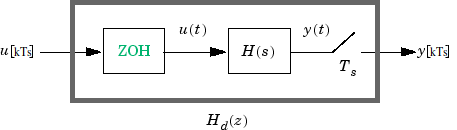
\includegraphics[width=1\textwidth]{Controllo/zoh-apply.png}
\end{figure}
\noindent
Questa interconnessione "\textit{congela}" l'ultimo segnale discreto $ u(k T_s) $ ricevuto e lo ripropone come un segnale costante in ingresso al sistema continuo che evolve in maniera indipendente.\\
L'uscita $ y(k T_s) $ è la discretizzazione di $ y(t) $, campionata ogni $ T_s $ \footnote{$ T_s $ = Sampling Time}.
\begin{figure}[H]
	\centering
	\caption[Effetto sui segnali discretizzati con il metodo Zero-Order Hold]{Segnali discretizzati con il metodo Zero-Order Hold}
	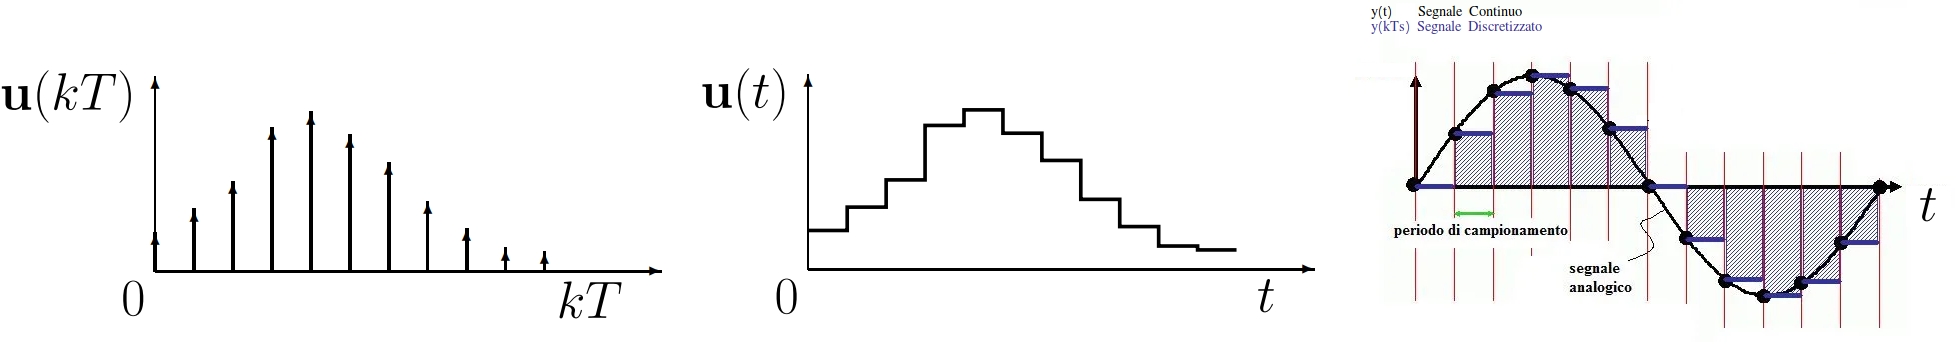
\includegraphics[width=1\textwidth]{Controllo/SegnaliDiscretiContinui.png}
\end{figure}
\noindent
Il sistema $ H(s) $ durante gli intervalli $ T_s $  evolve avendo una costante in ingresso, e al successivo istante di campionamento l'uscita raggiunta viene campionata e mantenuta per ul successivo $ T_s $, e questo procedimento all'infinito.
\newpage
\noindent
Ora che abbiamo descritto qualitativamente cosa avviene usando una discretizzazione ZOH, vediamo ora come diventa $ H_d(s) $ nello spazio di stato in termini matematici. Il procedimento di discretizzazione necessita di passare attraverso lo spazio di stato dei 3 sistemi dinamici che compongono il controllore \ref{eq:controllerDesign} e usando le formule del professore \cite{Discretizzazione}, si ottengono i risultati seguenti risultati:
\begin{table}[H]
	\centering
	\caption[Funzioni di trasferimento nello spazio di Stato, da Tempo Continuo a Tempo Discreto]{Funzioni di trasferimento nello spazio di Stato, da $ \mathbb{T} = \mathbb{R} \rightarrow \mathbb{T} = \mathbb{Z} $}
	{\LARGE \begin{tabular}[t]{||c||c||c||}
			\hline
			                                                                          &                                        &                         \\[-3mm]
			$ C_{I^2}(s) = \frac{K_2}{s^2}$                                           & $ C_I(s) = \frac{K_1}{s}$              & $ C_p(s) = K_p $        \\[2mm]
			                                                                          &                                        &                         \\[-3mm]
			{\normalsize $ \left\{\begin{matrix}
					\dot{x} = & \begin{pmatrix}
						0 & 1 \\
						0 & 0
					\end{pmatrix} x & + & \begin{pmatrix}
						0 \\
						K_2
					\end{pmatrix} u \\
					          &                                                               \\[-1mm]
					y       = & \begin{pmatrix}
						1 & 0
					\end{pmatrix} x
				\end{matrix}\right. $
			}                                                                         &
			$ \left\{\begin{matrix}
					\dot{x} = & x & + K_1 \cdot u \\
					y       = & x &
				\end{matrix}\right.$

			                                                                          &
			$\left\{\begin{matrix}
					y = K_p \cdot u
				\end{matrix}\right. $                                                                                                   \\[9mm]
			\hline\hline
			                                                                          &                                        &                         \\[-3mm]
			{\normalsize $ \left\{\begin{matrix}
					x^+ = & {\small \begin{pmatrix}
								1 & T_s \\
								0 & 1
							\end{pmatrix}} \cdot x_k & + & K_2 {\small \begin{pmatrix}
						T_s^2/2 \\
						T_s
					\end{pmatrix}} u_k \\
					      &                                                                                                \\[-1mm]
					y_k = & \begin{pmatrix}
						1 & 0
					\end{pmatrix} \cdot x_k
				\end{matrix}\right. $
			}                                                                         & {\normalsize
					$ \left\{\begin{matrix}
							x^+ = & x_k & + K_1 T_s \cdot u_k \\
							y_k = & x_k
						\end{matrix}\right.$

			}                                                                         &
			$\left\{\begin{matrix}
					y_k        = K_p \cdot u_k
				\end{matrix}\right. $                                                                                                  \\[9mm]

			                                                                          &                                        &                         \\[-3mm]
			$ C_{I^2}(z)|_{T_s} = K_2 \cdot \frac{T_s}{2} \cdot \frac{z+1}{(z -1)^2}$ & $ C_I(z)|_{T_s} = \frac{K_1 T_s}{z-1}$ & $ C_p(z)|_{T_s} = K_p $ \\[2mm]
			\hline
		\end{tabular}}
\end{table}
\noindent
I calcoli della trasformata Zeta, sono presenti solo per completezza e sono stati ottenuti usando la classica formula:
{\large \begin{center}
	$ G(z) = C_d \left(z I - A_d\right)^{-1} B_d + D_d $
\end{center}
}
%lst:controlLoop

\section{Codifica del controllore}

\section{Tuning delle costanti}

\section{Esperimenti}